%!TEX root = thesis.tex
\chapter{Implementation} % (fold)
\label{ch:implementation}
This section describes the implementation of the design choices made in the two previous chapters in terms of client side and server side tasks.

The proposed design presented in the previous chapter has accounted for the presented requirements and user needs, but there are some requirements that will not be implemented due to prioritisation.

Chapter~\ref{ch:design1} and \ref{ch:design2} presented an application that accounted for a user model, this chapter will only present how to collect the necessary user data and use it in the application -- and not implement it. It will, however, describe which metadata is needed and how to acquire it.

The social aspects is an important part of the system are also useful channels for awareness. \cite{Tidwell} even states her editorial mix pattern as a social media pattern. Nonetheless, these will not be implemented in the presented application as it does not contribute with new knowledge to the field. The gathered news articles to be used in this project contains both images and videos, but only images will be considered here. It is however trivial to implement support for videos as the same space allocation principles applies, but it was not prioritised.

Also, the personalised summaries have already been very well explored in \cite{fulltext.pdf} and this project will not try to compete with this solution, so only the first few sentences will constitute the excerpts from articles to be used on the front page. Because the full articles are shown in the sections no excerpts will be used in these. This should, however, be supported in the further development of the application.

The sections are based categories. These are by no means complete and they have not been verified. However, they are some of the most recurring in popular news sites and are used in order to proof the concept is possible. Thus, their definitions are not comprehensive either.

Finally, only a subset of the editorial mix constraints, presented in the Constraint Programming chapter (chapter~\ref{ch:design2}), will be implemented. Furthermore, before the user test was done the implementation had already started. This led to the implementation of a fairly complex layout constraint to minimise white space. It turned out that some white space was actually a user preference, but the implementation of the constraint will be presented nonetheless, as it shows a good example of what is possible with the system. 
%
%Whitespace between articles should be minimised. This is not an actual user requirement, but it is included as it a fairly complex layout problem to solve and it shows some aspects of what it can do.
\clearpage
%\section{Server for Acquiring and Mining Data for Personalisation}
\section{Similarity and Relevance {Computation}}
%\subsection{spatial, temporal and relational personalisation}
The \cite{DCMI} proposes 15 metadata elements for documents:
\begin{itemize}\itemdist
	\item Title
	\item Creator
	\item Subject
	\item Description
	\item Publisher
	\item Contributor
	\item Date
	\item Type
	\item Format
	\item Identifier
	\item Source
	\item Language
	\item Relation
	\item Coverage
	\item Rights
\end{itemize}
The articles in this project have been acquired using the Readability API\sidenote{An API to parse articles from websites.} to scrape articles given by links from RSS-feeds. This way it is possible to get the full article. Under normal circumstances, these would probably be supplied by a content provider, say through agreements with newspaper companies or social networks. The Readability API provides several metadata elements for the parsed articles; a domain, a title, an article URL, a lead image, the author, an article excerpt, a word count and a date of publication. This satisfies many of our needs, but there are still some very crucial calculations to be done, i.e.\ the article relevance according to user topics and similarity between articles.

The analysis of article relevance and similarity to other articles will use the same analysis, namely a keyword analysis using the WordNet and entity comparison using the Open Calais API\sidenote{A service by Thomson Reuters that automatically extracts semantic information from web pages in a format that can be used on the semantic web.}. These will be presented in the following.

WordNet is a large lexical database of English words and their relationships in the form of different graphs. WordNet is based on \emph{synsets}, which is a set of synonyms that describes different meanings of the same word. WordNet has a hyperonymy and hyponymy graph for noun synsets, which is based on the ISA relation between words. A \emph{hypernym} relation is a generalisation, e.g.\ a hypernym for a bed is a piece of furniture; and a \emph{hyponym} relation is a specification, e.g.\ a hyponym for a bed is a bunkbed. For nouns there also exists the meronymy graph, which is a graph describing the part-whole relation; a chair e.g.\ has a back, a seat and legs. Also, parts are inherited by superordinates, e.g.\ if a chair has legs, then an armchair has legs as well. Furthermore, WordNet has a graph describing elaboration, i.e.\ \emph{troponyms}, of verbs synsets, adjectives organised in terms of antonymy and adverbs which can be be described in terms of adjectives. The synsets, the hypernym and hyponym graph and the troponym graph of WordNet are the most interesting, because they describe different meaning of a given word, whereas the others describes relation to other words.
%Noun hyperonymy, hyponymy or ISA relation
%Noun Meronymy, inherited
%Verb synsets, troponyms: dimensions along which verbs can be elaborated
%Adjectives are organized in terms of antonymy
%adverbs are straightforwardly derived from adjectives via morphological affixation

The initial approach involved computing the TF-IDF similarity using the Python libraries for this \cite{NLTK}. This approach works on a bow (bag-of-words) with keywords and weights representing a single item. The weight is computed by the number of occurrences in the provided text and a cosine of the angle between them determines the similarity. However, Python also provides an interface for working with WordNet. This allows for a more in-depth analysis of the obtained news articles. \cite{116262780379.pdf} presents an algorithm for enriching articles using WordNet's hypernym graph, which proves to yield precise results in the context of enhancing labelling using K-means clustering. However, only the WordNet enriching of articles will be used to aid the keyword based approach in this implementation. In the presented approach a subgraph of WordNets hypernym graph is generated by the top $20\%$ frequent keywords of an article and weighted by equation~\ref{eq:weight}
\begin{align}
W(d, f) = 2 \cdot \frac{1}{1+e^{-0.125(d^3\frac{f}{TW})}}-0.5
\label{eq:weight}
\end{align}

Where $d$ stands for the node's depth in the graph (starting from root and moving downwards), $f$ is the frequency of appearance of the node to the multiple graph paths and $TW$ is the total number of words used to generate the hypernym graph. An example of such a hypernym graph is seen in Figure~\ref{fig:hypernym-graph}.
\begin{figure}[h!tp]
	\myfloatalign
	%\makebox[\textwidth][l]{
		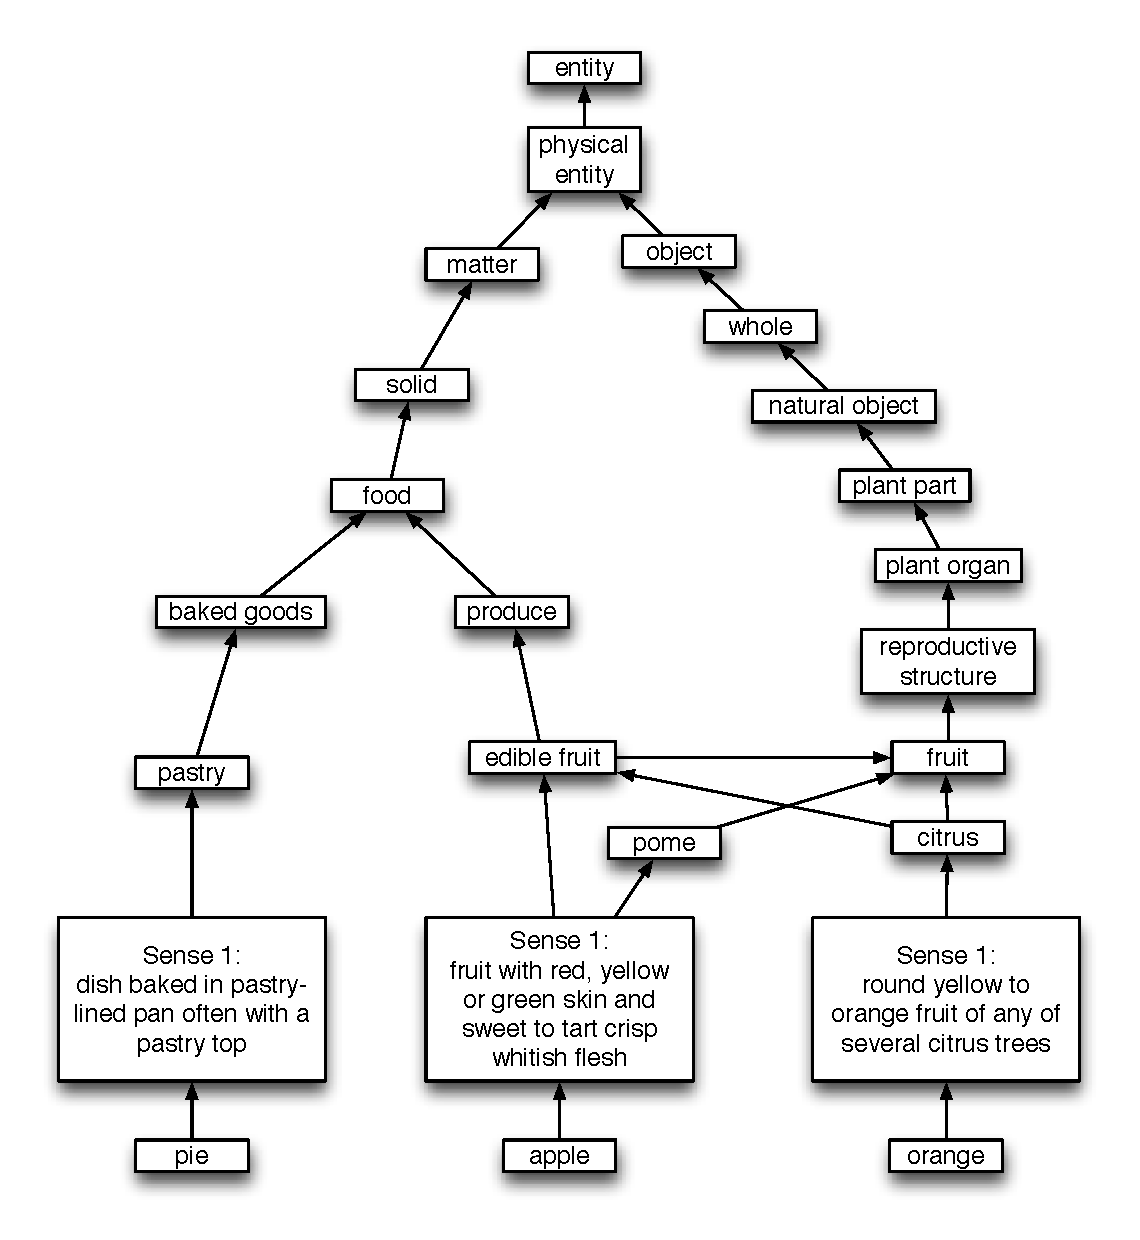
\includegraphics[width=.8\textwidth]{img/hypernym-graph}
	%}
	\marginnote{
		\begin{minipage}{\marginparwidth}
			\vspace{-250pt}
			\caption{The figure shows an example of a hypernym graph that could be generated by the \textsc{WordNet-Enrich}\\ algorithm.}
			\label{fig:hypernym-graph}
		\end{minipage}
	}
\end{figure}

To be able to work with hypernyms, words from articles must be converted to synsets. For each word there exists a synset for each use of the word, with the most frequently used first. Every synset is included in the analysis of this implementation, but in a later stage this could be further focused by only using the top $n$ uses of the word. In the algorithm given by \cite{116262780379.pdf} only the most general use is included (see Figure~\ref{fig:hypernym-graph}), which is a rough assumption. By this it is assumed that the meaning of every word extracted from an article is of the most general use. A better solution would be to use the Wu-Palmer similarity to find the best match of words (\cite{Wu-Palmer}). Wu-Palmer calculates a similarity based on the lowest common ancestor in the hypernym graph, which is available through the Python implementation. This way a set of keywords is gathered based on their most frequently common uses, as opposed to their independently common uses.

WordNet distinguishes among Types (common nouns) and Instances (proper nouns)\sidenote{Common nouns are general words for any people, places and things while proper nouns are specific names of individual people, places, things, or a title.}, so it is possible to extract these from the articles to base the analysis on. Both nouns and adjectives are extracted from articles, but adjectives could also be derived from adverbs to add meaning. A hypernym graph is produced of a maximum of 9 levels up in the graph and each of these synsets are weighted and the top $20\%$ extracted hypernymns along with the top $20\%$ of the original given keywords constitutes the final set of keywords, see Figure~\ref{fig:wordnet_enrich}.
\begin{figure}[ht!p]
	\hspace{-40pt}
	\newsavebox{\wordnetenrichbox}
	\begin{lrbox}{\wordnetenrichbox}
	\begin{minipage}{.75\largefigure}
		\vspace{-5pt}
		\begin{codebox}
\zi \proc{WordNet-Enrich}($a$) \kw{returns} enriched list of keywords
    \Indentmore
\zi \kw{inputs:}
    \Indentmore
    \zi $a$, an article \End
\zi $total\_hypernym\_graph \leftarrow$ a new graph
\zi $kws \leftarrow$ fetch $20\%$ most frequent kws for a
    \zi \For \kw{each} keyword $kw$ in $kws$ \kw{do} \Do
    \zi 	$hgraph \leftarrow$ \proc{WordNet-HypernymGraph($kw$)}
    \zi 	\For \kw{each} hypernym $h$ in $hgraph$ \kw{do} \Do
    \zi			add 1 to frequency of $h$ in $total\_hypernym\_graph$ \End \End
    \zi \For \kw{each} hypernym $h$ in $total\_hypernym\_graph$ \kw{do} \Do
    \zi     $d \leftarrow$ calculate depth of $h$ in WordNet hypernym graph
    \zi     $f \leftarrow$ frequency of $h$
    \zi     $weight \leftarrow 2 \cdot \frac{1}{1+e^{-0.125(d^3\frac{f}{\proc{size($kws$)}})}}-0.5$ \End
    \zi \proc{sort-weights($total\_hypernym\_graph$)}
    \zi $important\_hypernyms \leftarrow$ top $\frac{\proc{size($kws$)}}{5}$ of $total\_hypen\_graph$
    \zi \Return $kws \leftarrow kws + important\_hypernyms$
    \End
		\end{codebox}
		\vspace{-5pt}
	\end{minipage}
	\end{lrbox}\fbox{\usebox{\wordnetenrichbox}}
	%\marginnote{
	%	\begin{minipage}{\marginparwidth}
			\caption{The \proc{WordNet-Enrich} algorithm for enriching articles using hypernym graphs from WordNet, inspired by~\protect\cite{116262780379.pdf}.}
			\label{fig:wordnet_enrich}
	%	\end{minipage}
	%}
\end{figure}

After this extraction the similarity is computed by a path similarity, which is based on the shortest path between the words, on the best matches between words. The Wu-Palmer similarity, could again, be used instead, but to avoid more computation time the naïve solution was chosen.

Because it is possible to distinguish between proper nouns and common nouns in WordNet as well, this was used to extract instances from articles. However, WordNet often seemed to have problems with this particular issue and would, e.g.\ match an article about an exhibition of Claude Monet's flower garden to a topic containing the company Apple inc.
\begin{figure}[h!tp]
	\myfloatalign
	\subfloat{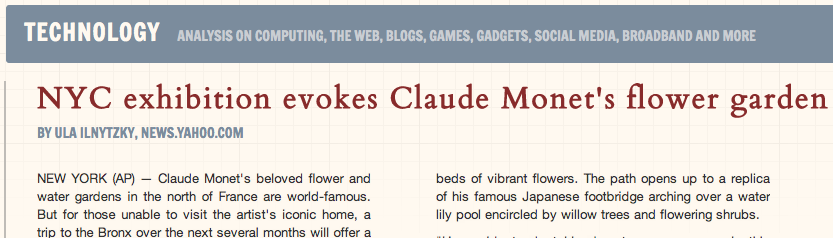
\includegraphics[width=.5\largefigure]{img/monet-small}}%
	\\
	\subfloat{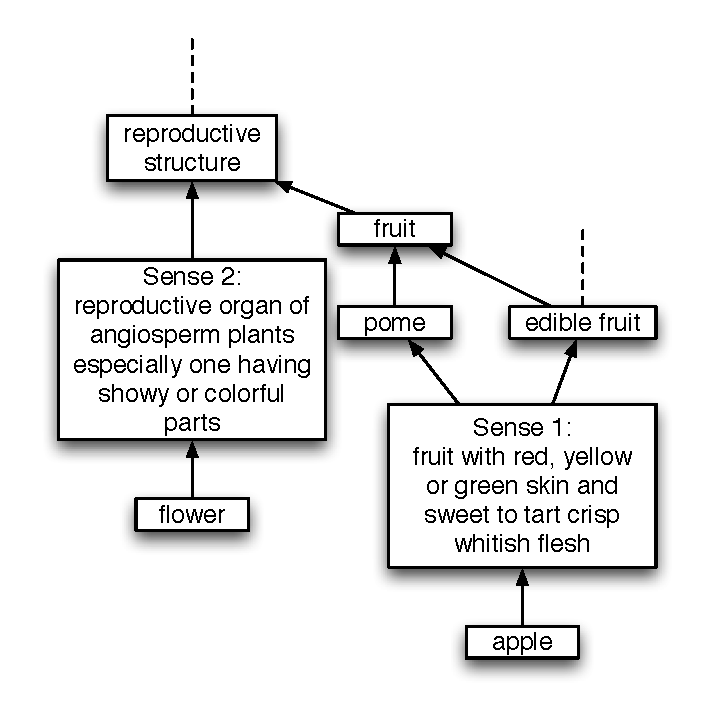
\includegraphics[width=.5\largefigure]{img/flower-apple}}%
	%\makebox[\textwidth][l]{
		%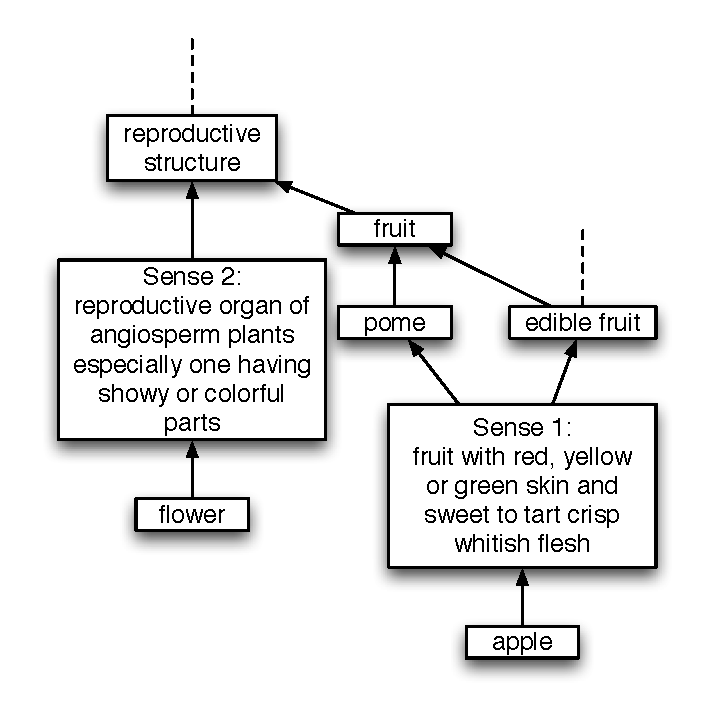
\includegraphics[width=.5\textwidth]{img/flower-apple}
	%}
	\marginnote{
		\begin{minipage}{\marginparwidth}
			\vspace{-370pt}
			\caption{The figure shows an example a close realtion in the hypernym graph of the words ``apple'' and ``flower''.}
			\label{fig:flower-apple}
		\end{minipage}
	}
\end{figure}

An example of where Wordnet does not perform well is New York. When the words are removed from each other, they provide another meaning, which is what the implementation supply WordNet with. But Open Calais can handle the full document and can detect where to keep the words together in order to find meaning.

To account for this a similarity using the Open Calais API was implemented.
%\todo[inline]{WordNet distinguishes among Types (common nouns) and Instances (specific persons, countries and geographic entities). (\url{http://wordnet.princeton.edu/})}
%\todo[inline]{level is only a part Python implementation of WordNet}

The Open Calais API provides analysis of documents and extraction of several kinds of metadata. This implementation will only use the extraction of entities, but it could however, be interesting to see how well the document categorisation performs, which includes many general news topics. After the extraction of entities the similarity is calculated by the sum of entity matches divided by the average length of the two given entity sets.

The final similarity is found by the average of the WordNet similarity and the entity similarity. This seemed to form a solid structure for computing the similarities between articles, but the relevance according to the user defined topics needs to be calculated as well. Fortunately, the decision of using keyword based user models lets us use the same functions to compute similarity between articles and topics. In Figure~\ref{fig:simplot} is a plot of similarities between articles and 9 different topics. The similarities are ordered by an average between them.
\begin{figure}[h!tp]
	\myfloatalign
	\makebox[\textwidth][l]{
		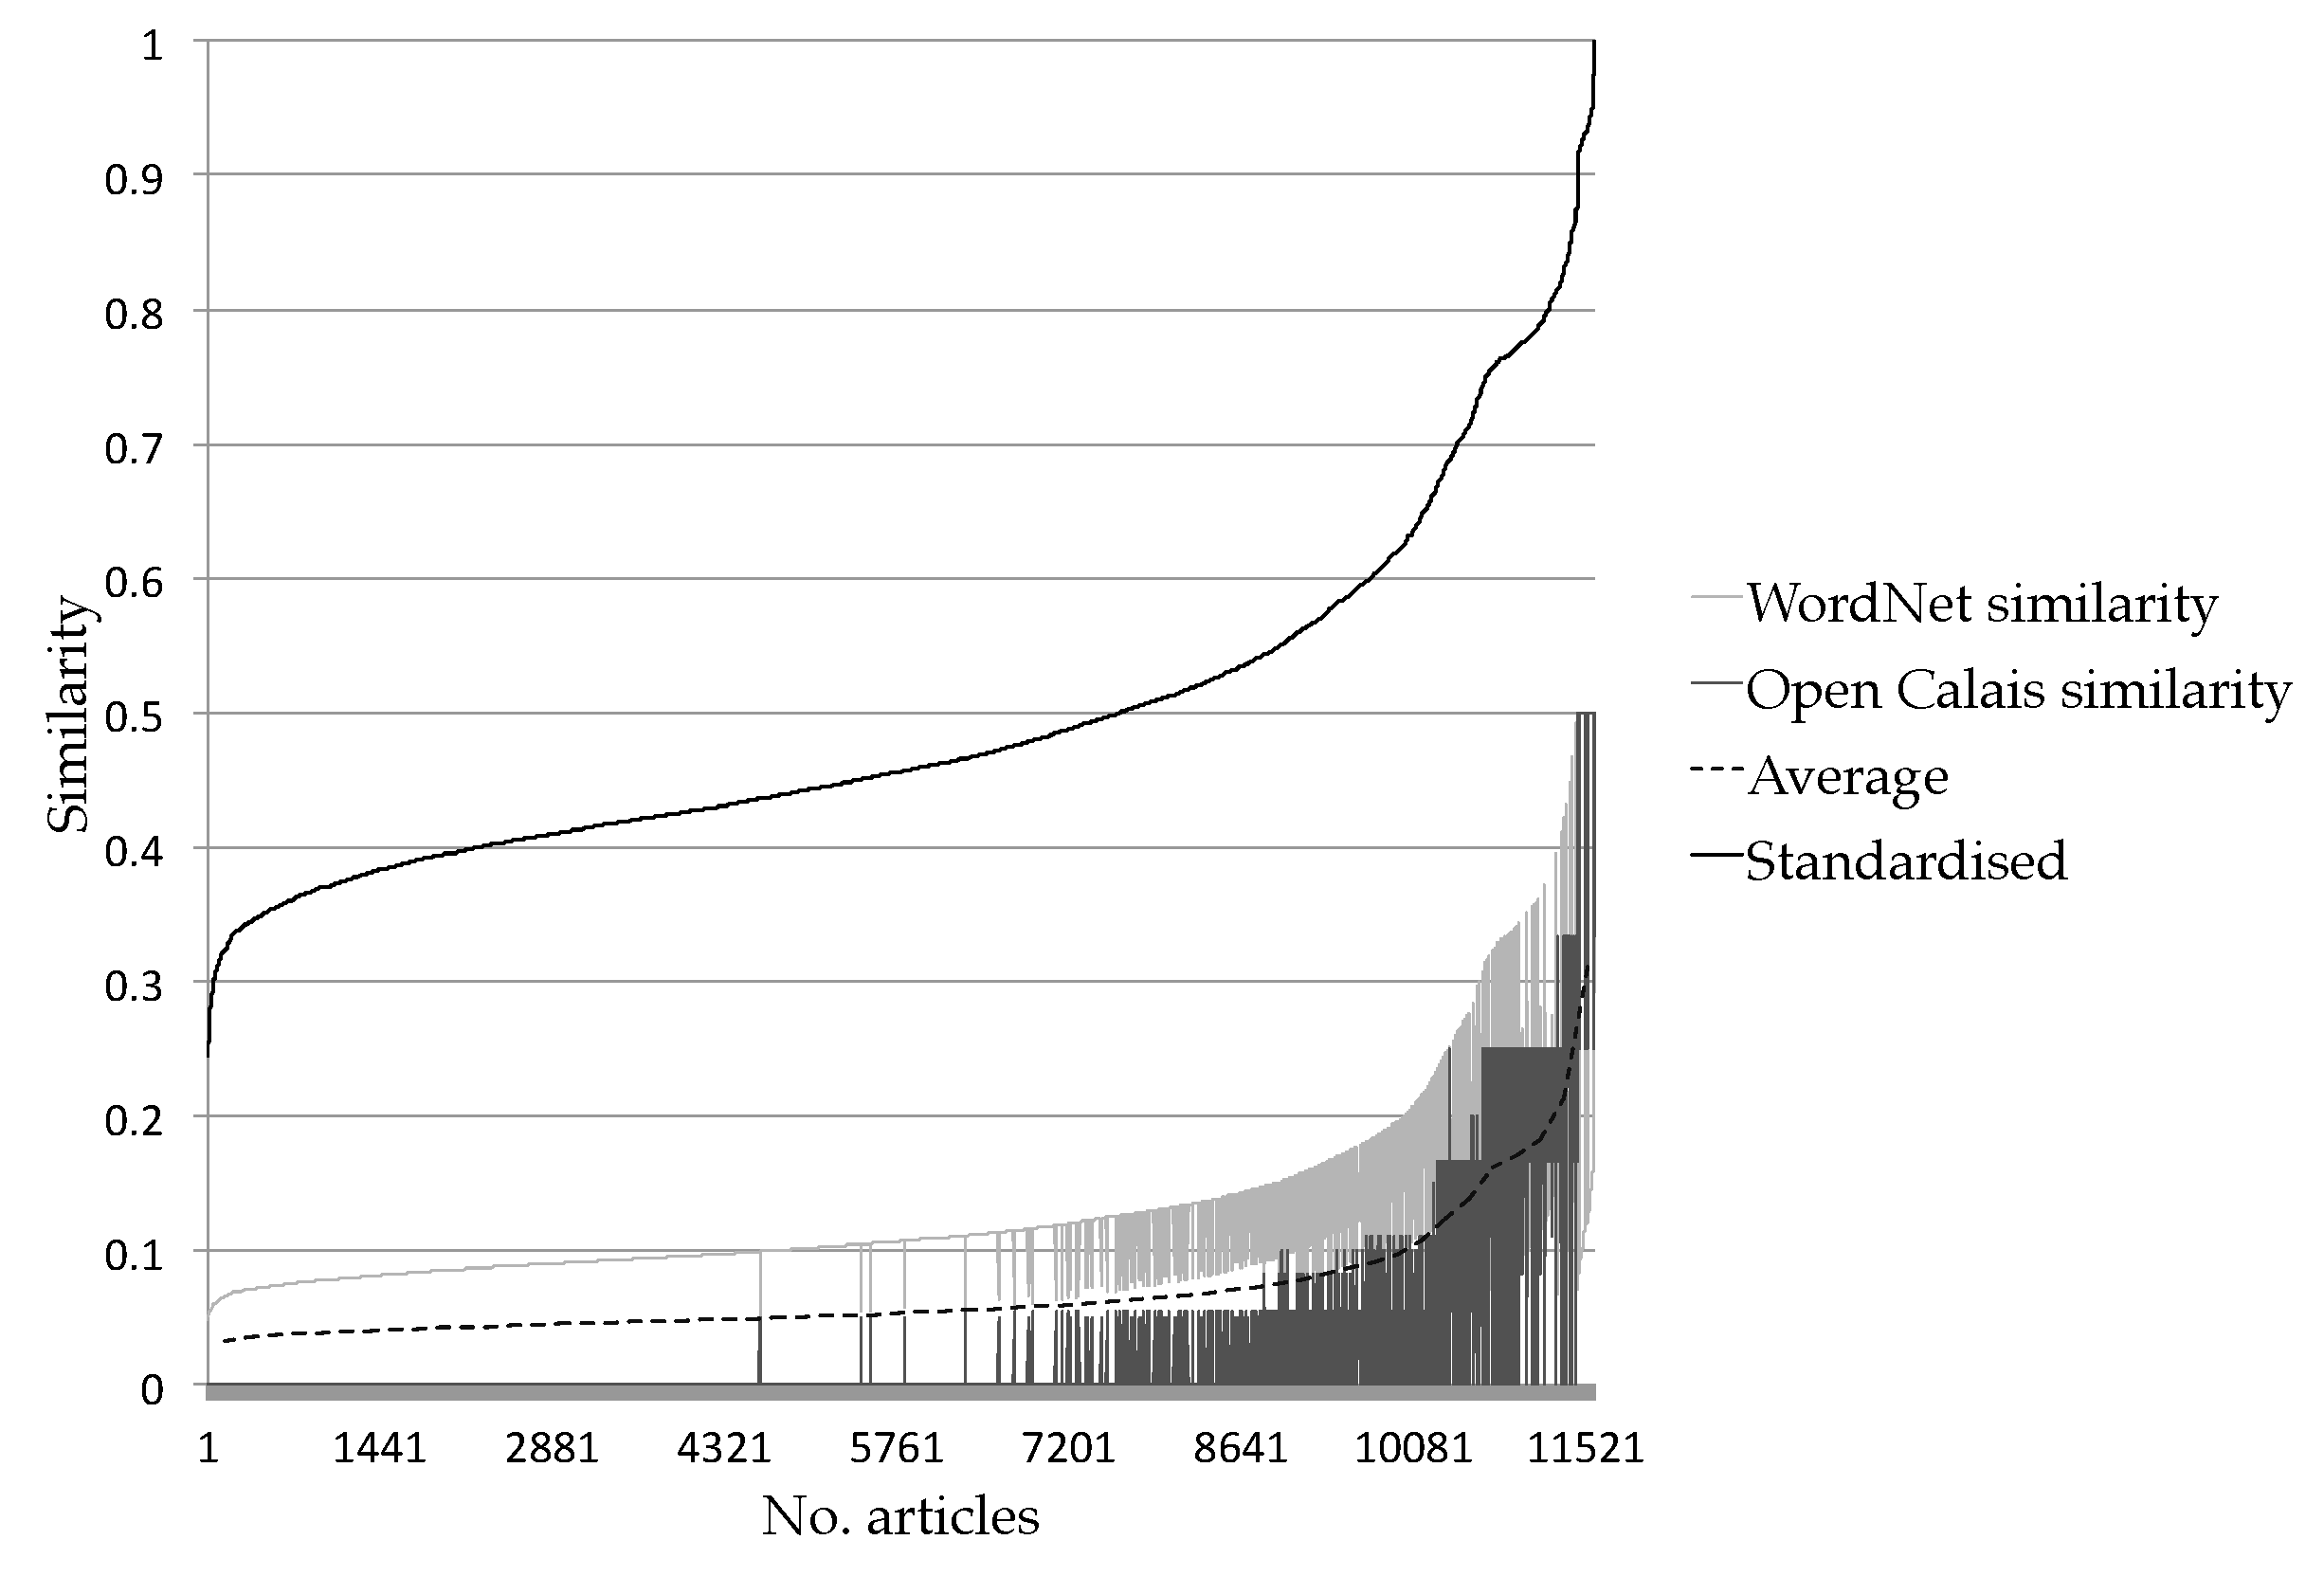
\includegraphics[width=.88\largefigure]{img/simplot}
	}
	\marginnote{
		\begin{minipage}{\marginparwidth}
		\vspace{-120pt}
			\caption{The figure shows a plot of articles with WordNet and Open Calais similarities, their average and a plot of the standardised average.}
			\label{fig:simplot}
		\end{minipage}
	}
\end{figure}

These similarities between articles, worked well but was somewhat strict. The highest similarity given was $0.396$ in a range of $[0;1]$. $86\%$ of them was below $0.1$. Because of this and that even fairly low similarities yielded promising results it seemed appropriate to standardise it. This is also plotted in Figure~\ref{fig:simplot}. The standardising of the data is done by taking the logarithmic function of their percentages to flatten it more and dividing it by the largest similarity to spread it evenly over the $[0;1]$ scale.

The articles are stored in a file on the server for easy retrieval by the client side and the metadata is stored in a database. The articles could have been stored in a database along with the metadata for a more sustainable solution, but this was just an easy solution.
%\subsection{Computing Similarity}
%- Storing Data

%\section{Client for Composing the Editorial Mix and Presenting the Articles}
\section{Interface}
In order to fulfil the requirements of a column based interface it seemed appropriate to use a grid based layout. Twitter Bootstrap\sidenote{A collection of tools for creating web applications.} provides an excellent framework for this which is both touch friendly and responsive\sidenote{Responsive Web Design means that the layout is adaptable to the viewing devices screen size.}. A layout was developed using conditional styling so an article can be assigned a class according to its size in columns so the layout can adapt to display the article differently according to size. An article that uses 3 columns in landscape mode should necessarily only uses the available 2 columns in portrait mode. This also promotes the possibility of having articles that displays in 1 column in portrait and 2 columns in landscape and finally articles that display 1 column in both.

The calculation of how many columns an article should use was done as a preprocessing, first by the largest image found along with the article and next the number of characters in the article. Users from the test pointed out that images should be as large as possible, and this should therefore dictate the space allocated for the article.

There are different ways of displaying text in columns on the web, but one of the newcomers is CSS3 Multi Columns\sidenote{See \url{http://www. w3schools.com/css3/css3_multiple_columns.asp}.}, which introduces easy styling of text in balanced columns. It was chosen to use this technology to see what was possible with it and because it is a technology that is under development. This means that it is not possible at the moment to divide the columns or let, e.g.\ an image span a number of columns using styling. Either an object has to span all columns or be wrapped into one, but their respective functionality is however soon to be supported. One could manually implement the division of columns, but it was deemed unimportant for the project to investigate this further. This means that some white space beside images might occur and that columns continues with no division.
%\todo[inline]{css: conditional styling}

The main page of the application is created dynamically. User preferences are registered from the from submission and saved locally. If the view changes, the articles from the former section is removed and the new ones are inserted in their place. This provides the possibility of introducing animations between section changes and lazy load of the pages.

In Figure~\ref{fig:sequence} is shown a sequence diagram of what the system does in order to display the front page (or a section), when the user opens the application.
%\sidecaptionfigure{\textwidth}{img/sequence}{The figure shows a sequence diagram from when the user chooses a topic category until he can read articles from this topic. \texttt{secNum} is the section number to display (the front page is section 0), \texttt{userId} is a string that identifies the user, \texttt{userPrefs} is the user preferences on the specific section and \texttt{articles} is the library of articles to compose the editorial mix of.}{fig:sequence}
%\begin{figure}[h!tp]
%	\myfloatalign
%	\makebox[\textwidth][l]{
%		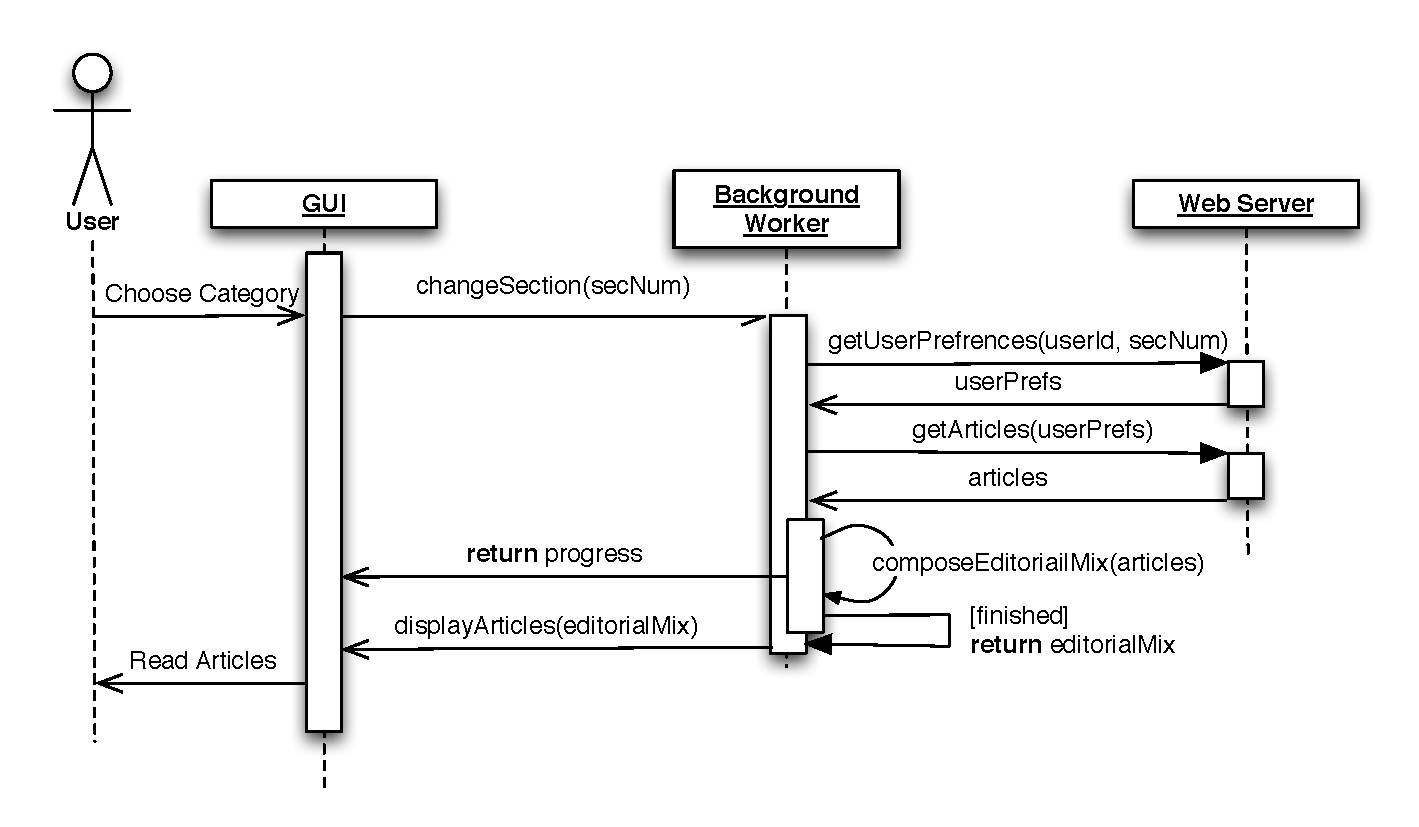
\includegraphics[width=.8\largefigure]{img/sequence}
%	}
%	\marginnote{
%	\vspace{-50pt}
%	\begin{minipage}{\marginparwidth}
%		\caption{A sequence diagram from when the user chooses a topic category until reading articles. \texttt{secNum} is a section number, (front page is section $0$), \texttt{userId} the user id, \texttt{%userPrefs} the user preferences on a given section and \texttt{articles} is a library of articles to compose the editorial mix of.}
%	\label{fig:sequence}
%		\end{minipage}
%	}
%\end{figure}
\begin{figure}[h!tp]
	\centering
	
	\def\mygraphic{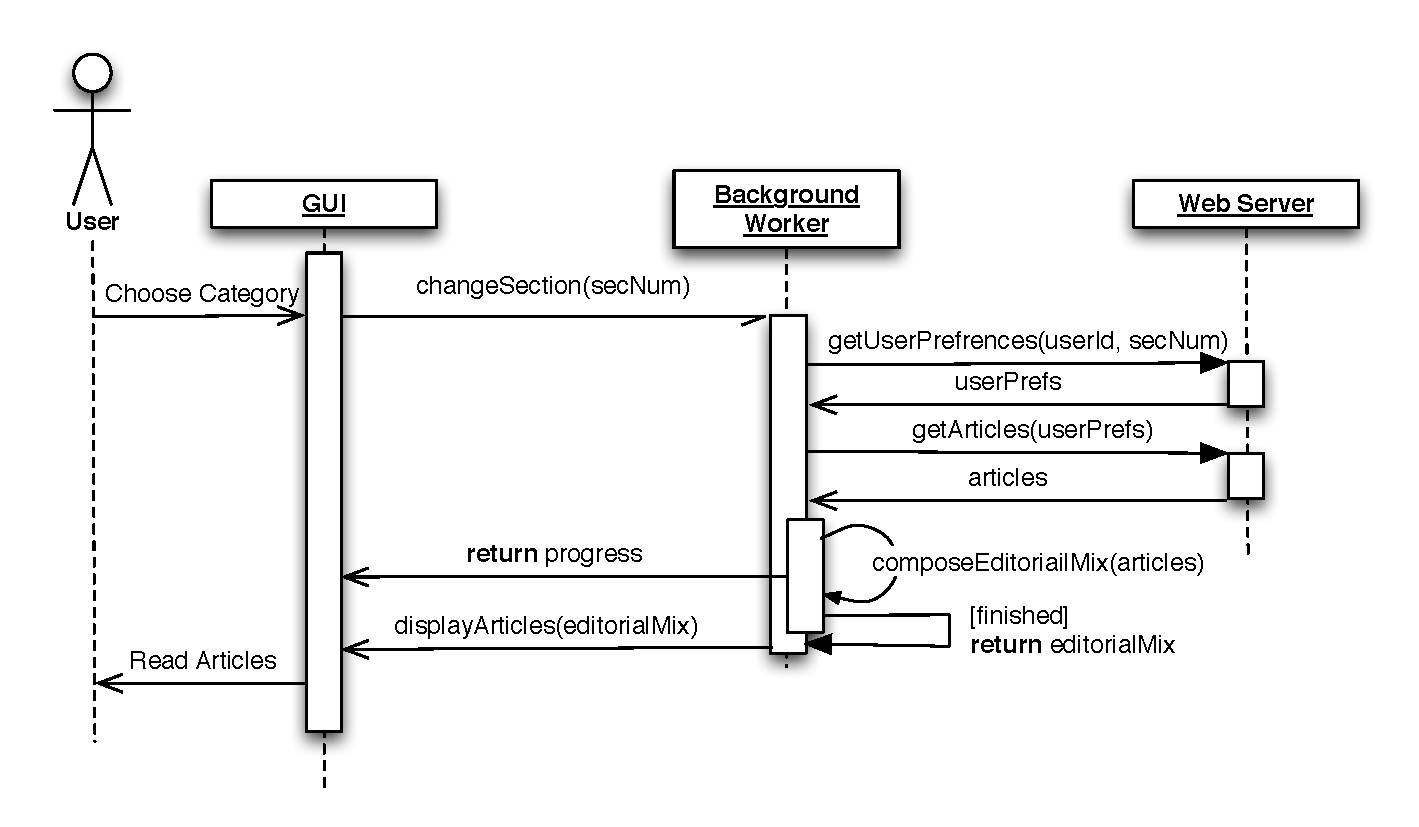
\includegraphics[width=\textwidth]{img/sequence}}
	%\newlength{\graphicheight}
	\settoheight\graphicheight{\mygraphic}
	\mygraphic
	\marginnote{
	\begin{minipage}{\marginparwidth}
		\vspace{-\graphicheight}%
		\caption{A sequence diagram from when the user chooses a topic until reading articles. $secNum$ is a section number, (front page is section $0$), $userId$ the user id, $userPrefs$ the user preferences on a given section and $articles$ is a library of articles used to compose the editorial mix.}
		\label{fig:sequence}
		\vspace{\graphicheight}
		\end{minipage}
	}
\end{figure}
%\begin{figure}[h!tp]
%	\myfloatalign
%		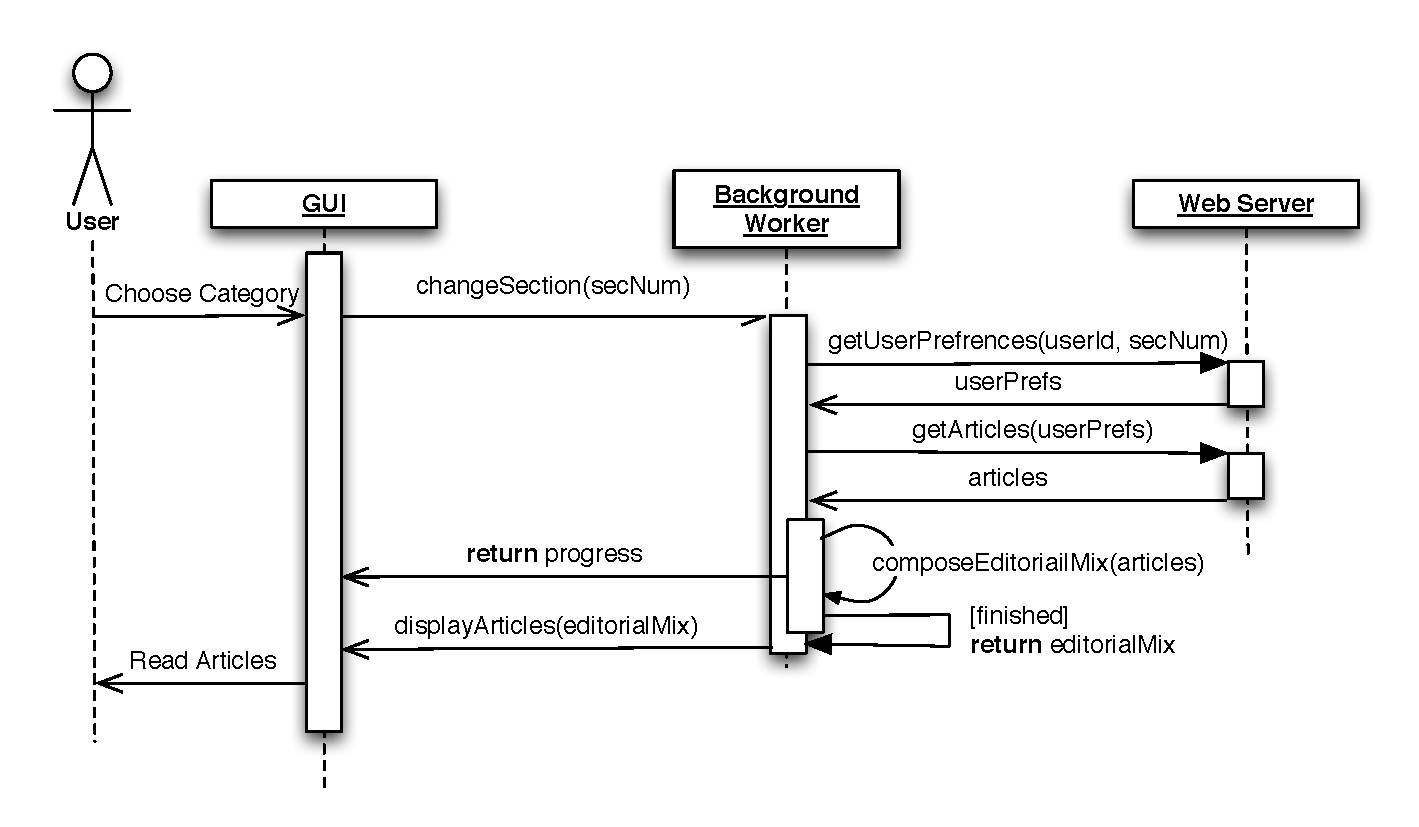
\includegraphics[width=\textwidth]{img/sequence}
%	\caption{The figure shows a sequence diagram from when the user chooses a topic category until he can read articles from this topic. \texttt{secNum} is the section number to display (the front page is section 0), \texttt{userId} is a string that identifies the user, \texttt{userPrefs} is the user preferences on the specific section and \texttt{articles} is the library of articles to compose the editorial mix of.}
%	\label{fig:sequence}
%\end{figure}

When the application is opened, or the application is changed to display a section, a background worker is initialised to compose a mix of articles. If the mix of articles in a section, or the front page, have already been computed, it should not have to recompute it. The background worker needs to get both the user preferences of the chosen topic and articles that potentially fit the user preferences. While the worker computes the editorial mix it sends messages to the user interface about the progress. This is used to provide feedback to the user. When it finishes the user interface is asked to display the articles.

The implementation does not log user behaviour and does not support relevance feedback to be stored in a user model. The user model have been manually written with manual definitions of keywords and their respective weights for sections. It was chosen not to focus on the logging of data to represent the user model, because it does not contribute with new knowledge to the field. The logging of data could, however, be done by detecting when an article enters the screen, e.g.\ using jQuery Waypoints\sidenote{A small jQuery plugin that makes it easy to execute a function whenever you scroll to an element.}. jQuery Waypoints provides events whenever an item enters the screen, then a time stamp could be registered and stored with a duration, when a new article enters the screen. Problems might, though, emerge when more articles are shown on the screen at the same time. Which article does the user read? A solution to this could be to register the touch, as the user might interact more with the screen in some places based on the position of the article he reads. This project will leave the problem to its field of study.
%\todo[inline]{Noget om hvordan programmet kunne samle keywords med vægte for en bruger?}

The next section will describe how the background worker handles its assigned tasks.

\section{Background Worker}
The choice of using a background worker to do the computation is essentially based on minimising the work for the UI thread. Web Worker\sidenote{A JavaScript script that runs in the background, independently of other, user-interface scripts that may also have been executed from the same HTML page.} introduces long-running JavaScript scripts which are not interrupted by scripts that respond user interactions, and allows long tasks to be executed without yielding to keep the page responsive. With this supporting browsers assigns a thread to handle the background worker tasks, but it remains in the same process.

Background workers are not meant to be numerous, because they require a high start-up performance cost and per-instance memory cost. On this basis a background worker was build to handle the section constraints and the front page constraints, respectively. In the further development it would make more sense to merge the two files, as they share a lot of code. It did however give a nice division between their respective assignments. When the user has submitted the form, as described in section~\vref{sec:layout_typography}, a background worker is asked to compute the editorial mix. It first creates the COP, with variables based on the user input, their respective domains and constraints to fit the section. Information is sent from the main script to the worker, so it can base the constraints on this, e.g.\ a list of articles from the front page is sent when a section should be composed. This way the knowledge is kept in the main script and shared amongst workers to be applied in specific problems. After the COP has been created it fetches potential articles and calls a library to do the constraint computation.

\section{Constraint Personalisation Library}
A library was developed for solving personalisation problems using CP. It was implemented using the \textsc{Min-Conflicts} algorithm along with the MCV heuristic to guide the selection of variables. The motivation for building the library comes from a need of a CP library that supports the use of a list of values consisting of real world items instead of having to define the items as a sub-problem. This section will describe how to use it and discusses the choices of implementation. The library is from here on referred to as \emph{Constraint Personalisation Library} or CPL\sidenote{The library can be downloaded here: \url{http://lestrade.imm.dtu.dk/~s062596/js/cp.js}.}.%the data structure, its general purpose solver

The library provides the possibility for creating a list of variables, with their respective domains and subdomains, see Table~\ref{code:domain}.
\begin{table}[h!tp]
\caption{Declaration of a domain, subdomain and variable}\label{code:domain}
\begin{lstlisting}{JavaScript}
var d = new Domain();
d.addSubdomain(
	// descrete domain (min, max, gap)
	new Subdomain(0, 1, 1),
	// subdomain name
	'images',
	// function for retrieving value attr
	function(x) {
		return x.images.length >= 1? 1: 0;
	}
);
// variable at position 0
var variable = new Variable(0,d);
cop.variables.push(variable);
\end{lstlisting}
\end{table}

After variables and domains have been declared it is possible to declare constraints on them, see Table~\ref{code:constraint}.
\begin{table}[h!tp]
\caption{Declaration of a constraint}\label{code:constraint}
\begin{lstlisting}{JavaScript}
var c = new Constraint(
	// constraint name
	'image0',
	// violation function
	function(vars) {
		if (vars[0] > 0) { return 0; }
		return 1;
	},
	// name of subdomain to work on
	'images',
	// variable positions to get
	// in the violation function
	[0]
);
cop.constraints.push([[c]]);
\end{lstlisting}
\end{table}

The constraints of the COP is stored in a list of lists of lists for two reasons. Firstly the nested list of nested lists is interpreted as a conjunction of disjunctions of conjunctions. The outermost conjunction is interpreted as the set of constraints, where the inner disjunction of conjunctions is interpreted as a decomposition of the constraint. This is to make it possible for the developer to declare a list of alternate sub-constraints as a decomposition of a constraint, i.e.\ it is possible for the user to declare a set of sub-constraints where either one of them should be fulfilled in order to satisfy the rule. This means that $[[[c_1,c_2],[c_3]],[[c_4]]]$ would be interpreted as $((c_1 \wedge c_2) \vee c_3) \wedge c_4$, where $c_1$ to $c_4$ are constraints.

An example of where this can be used is in the earlier described \texttt{image} constraint (see equation~\vref{eq:section_constraints}). This constraint is defined on 4 variables, where either one of them should have an image for the constraint to be fulfilled. Instead this could be described as a list of four lists with one constraint in each. Constraints that each looks like the one presented in the Table~\ref{code:constraint}, on variables in position 1 to 4, 4 to 7, 7 to 10, etc. There might also emerge situations where it could be useful to have alternating conjunctions of constraints. An example of this is the earlier mentioned white space minimisation, which is expressed as a more complex constraint.

The minimisation of white space can be expressed in terms of columns as; the accumulated sum of the columns assigned to articles in the problem in the next step minus the accumulated sum in the former step always be dividable with both 2 and 3. The following boolean expression expresses the same:
\begin{align*}
	&(sum_i-sum_{i-1} < 2 \vee sum_i-sum_{i-1}\ \texttt{\textbf{mod}}\ 2\ \neq 0) \wedge\\
	&(sum_i-sum_{i-1} < 3 \vee sum_i-sum_{i-1}\ \texttt{\textbf{mod}}\ 3\ \neq 0)
\end{align*}
Where \texttt{\textbf{mod}} is the modulus function.

In other words; any composition of articles should always fill out the screen in both portrait and landscape. Many possibilities for achieving this is available. For a list of three articles, this could be done by having three articles where each would have $2.5$ columns assigned. An article that is assigned $2.5$ columns means that is fills two columns in portrait and three in landscape, whereas an article assigned $1.5$ would display in one column in portrait and two in landscape. A more complex function could also describe the possibilities for two articles in a row, or three, or even more. The constraints could therefore be described as a disjunction of conjunctions as the following:
\begin{equation}
\begin{split}
[&[columns_0, columns_1, columns_2],\\
&[columns_{0-1}, columns_2],\\
&[columns_{0-2}]]
\end{split}
\label{eq:col-row}
\end{equation}
\begin{equation}
\begin{split}
((&columns_0 \wedge columns_1 \wedge columns_2) \vee\\
(&columns_{0-1} \wedge columns_2) \vee\\
&columns_{0-2})
\end{split}
\label{eq:col-row-logic}
\end{equation}
Where the number denotes which variable positions in the problem the constraint works on. A declaration of a white space minimising constraint over two variables is seen in Table~\ref{code:cols-constraint}.
\clearpage
\begin{table}[h!tp]
\caption{Declaration of a constraint for minimising white space}\label{code:cols-constraint}
\begin{lstlisting}{JavaScript}
var c = new Constraint('columns0-1',
	function(vars) {
		var violation = 0;
		if (vars[0] == 1) {
			if (vars[1] != 1.5) {
				violation++;
			}
		} else if (vars[0] == 1.5) {
			if (vars[1] != 1) {
				violation++;
			}
		} else {
			violation++;
			if (vars[1] != 1 && vars[1] != 1.5) {
				violation++;
			}
		}
		return violation;
	}, 'columns', [0,1]);
cop.constraints.push(c);
\end{lstlisting}
\end{table}

The second reason for this representation of constraints is that it is possible to declare constraints on fewer variable and that it is possible for the system to prune some calculations. The first constraint in a disjunction that evaluates to true, or in this case to violation $0$, makes it possible to discard the rest of the constraints in that disjunction. If the constraints are then ordered by how many variables they work on, so the system tries to evaluate the constraints in a conjunction that is defined on fewest values first, then it may never have to evaluate constraints that are global. In worst case it would have to evaluate all of them. An example of this ordering is seen in equation~\ref{eq:col-row} or \ref{eq:col-row-logic}, where the first nested list is only of unary constraints, the second a list of a binary and an unary and finally a single global constraint. However, it is also worth deciding how important it is that the application explores more complex solutions if simpler solutions works just as well. In any case it leaves the possibilities for the developer to optimise his definition of the problem. In further development it could be interesting to explore automatic reduction and organisation of constraints.

\cite{AIRussell} proposes constraint weighing to aid the organisation and furthermore maybe even lead the search to concentrate on variables that is bound by these constraints to solve them first. Constraints in this implementation are only represented as preference constraints, so every constraint returns a violation. This aids the search towards concentrating on changing variables that yields a lesser violation, but it also means that the returned assignment could violate constraints that are not supposed to be violated if the algorithm had trouble with finding a solution for the given problem. Using solely preference constraints eliminates the possibility of letting the search go on until a solution has been found. On the other hand one could argue, with a fixed budget computation problem, it is better to deliver the best assignment so far, than nothing at all.
%\subsection{Data Structure}
%\subsection{General Purpose Solver}
%Preference ordering of hard constraints or division between preference constraints and hard constraints.
%Assignment from library instead of arbitrary assignment? The latter is a more hypothetical approach. Providing the library as a constraint, where each variable assignment must have a unique combination from one of the possibilities of the constraint.
%(sim,breaking,chars,date,sections?,columns):list
%The former introduces an implicit constraint in that the general purpose solver can only choose from the library, thus can only choose a combination of values that exists.
%
%\todo[inline]{Ranges can be optimised in space by converting them to integer ranges. This can be done by setting min = 0 and max = (b-a)/gap.}
%The library could take any combination of constraints and then organise them into conjunctions of disjunctions, with the constraints taking fewer values first.
%In the implementation this is done by hand, so the program takes conjunctions of disjunctions of constraints organised with constraints that takes fewer values first. Constraint weighing could also help organising the disjunctions and furthermore lead the search to concentrate on variables that is bound by these constraints. (p. 222 AIRussel).
%
%\todo[inline]{Constraints should point to specific variables, this makes it somewhat rigid/ineffective because I have to write at global constraint that accounts for everything (ineffective in propagation -- might also be a problem if it does not show progress in changing values, i.e.\ it is a hard constraints and not returning a cost of the set of values.) or divide it into smaller constraints separated by an `or' (v). The latter is ineffective because there would should be a combination of constraints accounting for every situation, e.g. if the first variable is satisfying an unary constraint, the next say 3 variables (if the problem holds 4 variables) could satisfy three unary constraints, an unary and a binary (two combinations exists) or a constraint that takes three variables. This grows fast with the number of constraints.}
%
%\todo[inline]{Does it make sense that a continuous range cannot have specific values removed? Should it be possible for it be divided into subranges if the user decides to remove a range of values in between its domain of [min;max]?}

Constraints that have been implemented to compose the sections are \texttt{all-diff}, \texttt{fp-articles}, \texttt{topic}, \texttt{main-stories}, \texttt{adj-subj}, \texttt{images} and constraints to minimise white space. Also, the \texttt{featured-image} and \texttt{nonfeatured-image} have been implemented, but only as the same constraint that prefers images on every article, meaning that there is not a distinction between featured and non-featured articles.

Screenshots of the final implementation is seen in Figure~\ref{fig:screenshots} and can be accessed on \url{http://lestrade.imm.dtu.dk/~s062596}.

\begin{figure}%
%\centering%
\makebox[\textwidth][r]{% %%% as above; this time, the
%%% figures flushes from the left
\subfloat[Screenshot of the form.\label{fig:screenshot1}]%
	{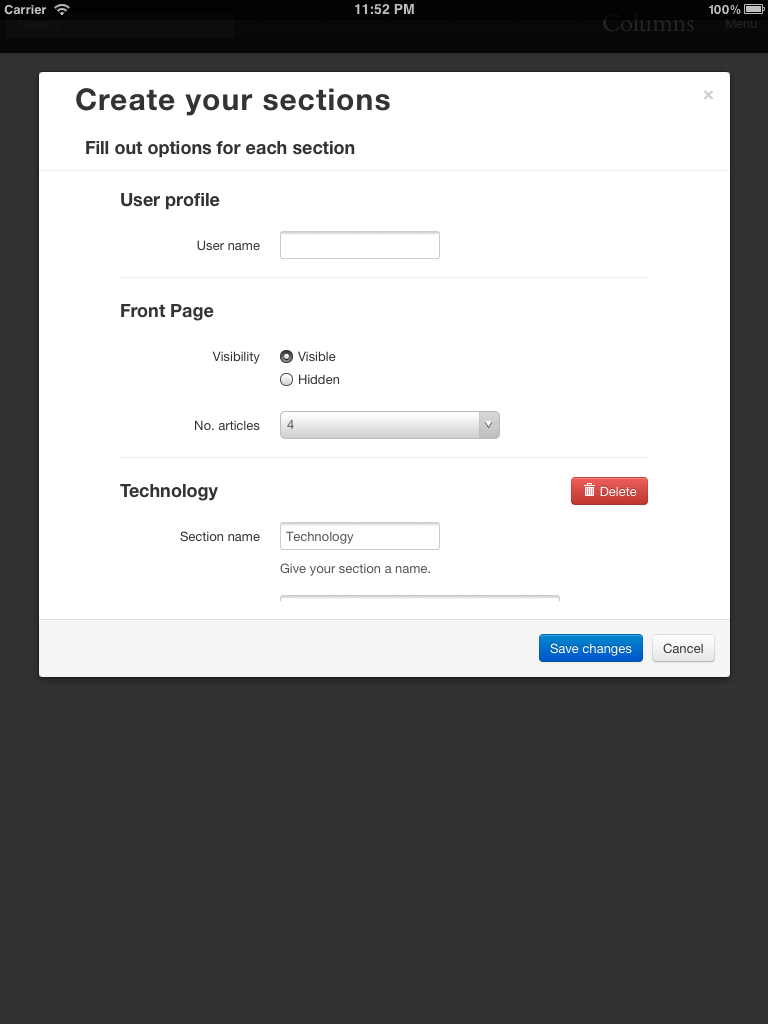
\includegraphics[width=.33\largefigure]{img/screenshot1}}%
	\qquad%
\subfloat[Screenshot from the sports section.\label{fig:screenshot2}]%
	{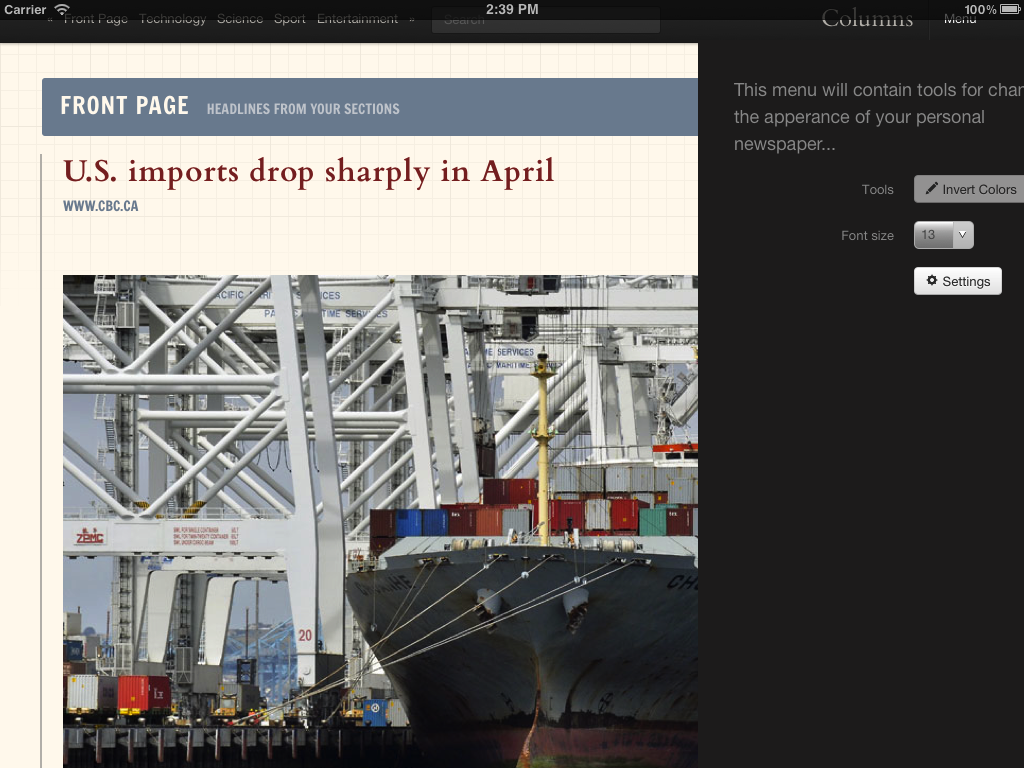
\includegraphics[width=.43\largefigure]{img/screenshot2}}%
}
\\
\makebox[\textwidth][r]{% %%% as above; this time, the
\subfloat[Screenshot from the technology section (portrait).\label{fig:screenshot3}]%
	{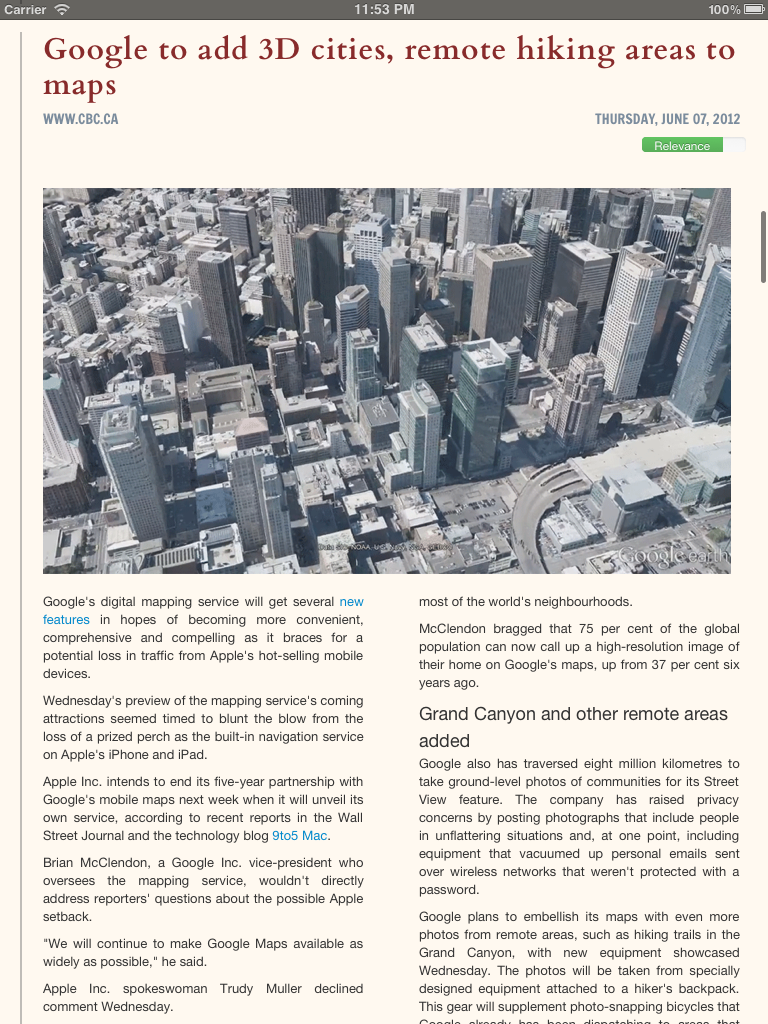
\includegraphics[width=.33\largefigure]{img/screenshot3}}%
	\qquad%
\subfloat[Screenshot from the technology section (landscape).\label{fig:screenshot4}]%
	{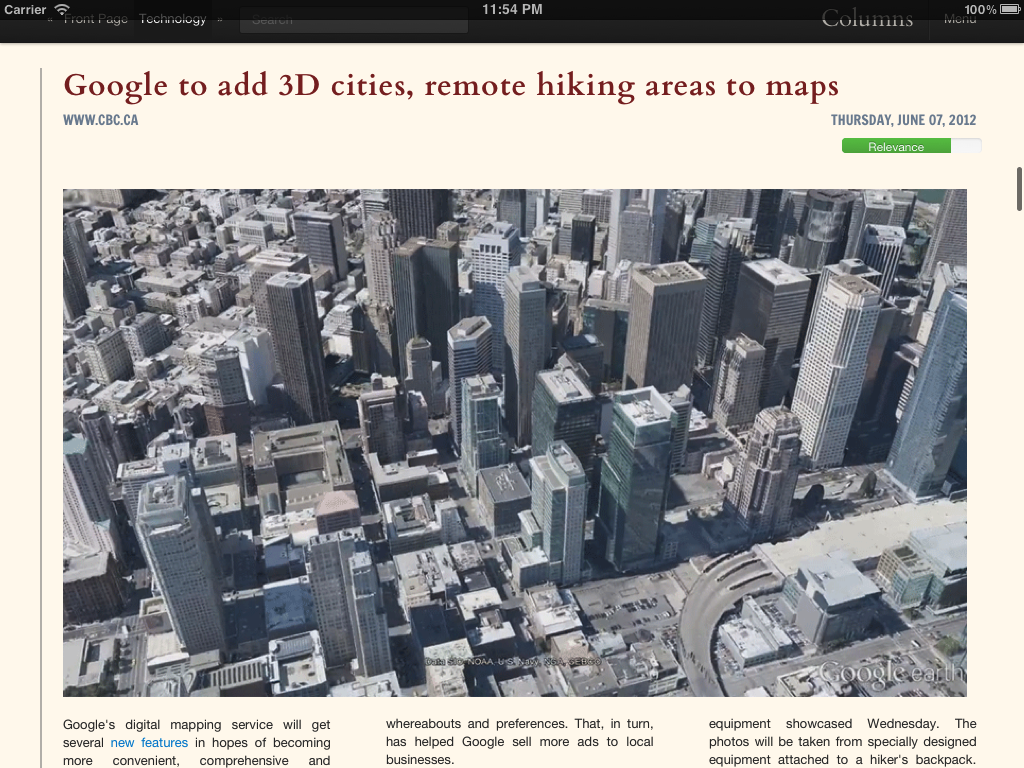
\includegraphics[width=.43\largefigure]{img/screenshot4}}%
}
\caption{The figure shows four screenshots of the final implementation.}%
\label{fig:screenshots}%
\end{figure}

The next chapter will evaluate the solution in terms of quality and performance.

% section design (end)